\documentclass[
  captions=tableheading,
  bibliography=totoc, 
  titepage=firstiscover,
]{scrartcl}

\usepackage{blindtext} %neuer input

\usepackage{longtable} % Tabellen über mehrere Seiten

\usepackage[utf8]{inputenc} %neuer input

\usepackage{scrhack}

\usepackage[aux]{rerunfilecheck} %Warnung falls nochmal kompiliert werden muss

\usepackage{fontspec} %Fonteinstellungen

\recalctypearea{}

\usepackage[main=ngerman]{babel} %deutsche Spracheinstellung

\usepackage{ragged2e} %neuer input

\usepackage{amsmath, nccmath}

\usepackage{amssymb} %viele mathe Symbole

\usepackage{mathtools} %Erweiterungen für amsmath


\DeclarePairedDelimiter{\abs}{\lvert}{\rvert}
\DeclarePairedDelimiter{\norm}{\lVert}{\rVert}

\DeclarePairedDelimiter{\bra}{\langle}{\rvert}
\DeclarePairedDelimiter{\ket}{\lvert}{\rangle}

\DeclarePairedDelimiterX{\braket}[2]{\langle}{\rangle}{
#1 \delimsize| #2
}

\NewDocumentCommand \dif {m}
{
\mathinner{\symup{d} #1}
}


\usepackage[
  math-style=ISO,
  bold-style=ISO,
  sans-style=italic,
  nabla=upright,
  partial=upright,
  warnings-off={
    mathtools-colon,
    mathtools-overbracket,
  },
]{unicode-math}

\setmathfont{Latin Modern Math}
\setmathfont{XITS Math}[range={scr, bfscr}]
\setmathfont{XITS Math}[range={cal, bfcal}, StylisticSet=1]


\usepackage[
  locale=DE,
  separate-uncertainty=true,
  per-mode=reciprocal,
  output-decimal-marker={,},
]{siunitx}

\usepackage[autostyle]{csquotes} %richtige Anführungszeichen

\usepackage{xfrac}

\usepackage{float}

\floatplacement{figure}{htbp}

\floatplacement{table}{htbp}

\usepackage[ %floats innerhalb einer section halten
  section,   %floats innerhalb er section halten
  below,     %unterhalb der Section aber auf der selben Seite ist ok
]{placeins}

\usepackage[
  labelfont=bf,
  font=small,
  width=0.9\textwidth,
]{caption}

\usepackage{subcaption} %subfigure, subtable, subref

\usepackage{graphicx}

\usepackage{grffile}

\usepackage{booktabs}

\usepackage{microtype} %Verbesserungen am Schriftbild

\usepackage[
backend=biber,
]{biblatex}

\addbibresource{../lit.bib}

\usepackage[ %Hyperlinks im Dokument
  german,
  unicode,
  pdfusetitle,
  pdfcreator={},
  pdfproducer={},
]{hyperref}

\usepackage{bookmark}

\usepackage[shortcuts]{extdash}

%\usepackage{warpcol}

\allowdisplaybreaks

\begin{document}
    \title{Physik IV Übungsblatt 4}
    \author{  
    Tobias Rücker\\
    \texorpdfstring{\href{mailto:tobias.ruecker@tu-dortmund.de}{tobias.ruecker@tu-dortmund.de}
    \and}{,} 
    Paul Störbrock\\
    \texorpdfstring{\href{mailto:paul.stoerbrock@tu-dortmund.de}{paul.stoerbrock@tu-dortmund.de}}{}
    }
\maketitle
\center{\Large Abgabegruppe: \textbf{4H}}
\thispagestyle{empty}

\newpage
\tableofcontents
\thispagestyle{empty}
\newpage

\setcounter{page}{1}

\section{Aufagabe 1}

    \begin{figure}[H]
        \centering
        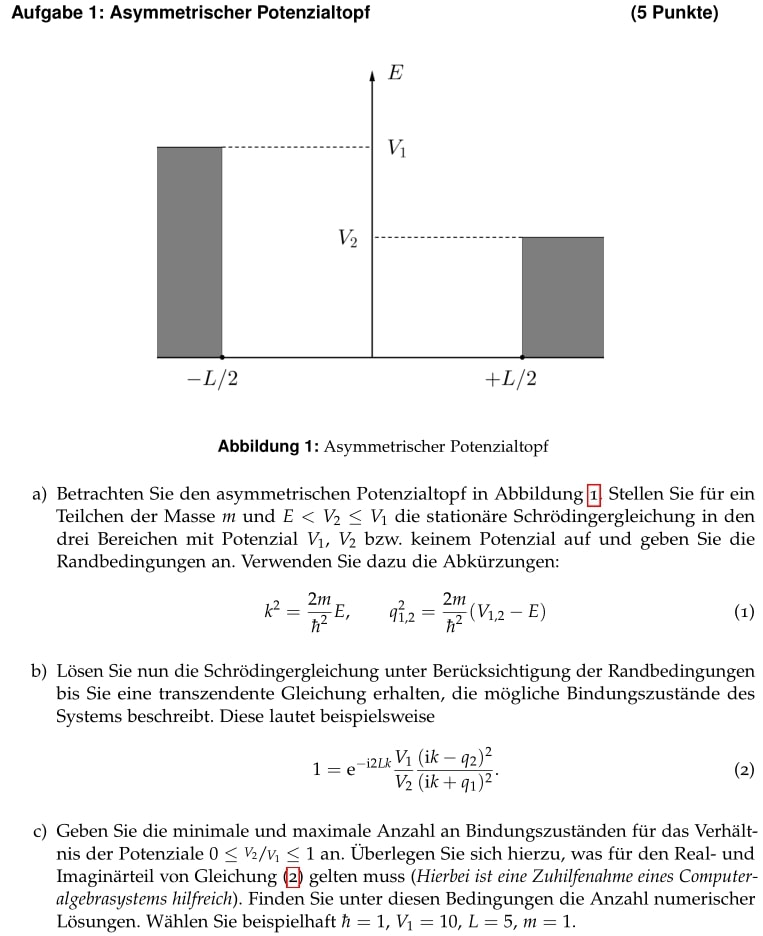
\includegraphics[width=\linewidth]{images/Aufgabe1.jpg}
        \label{fig:1}
    \end{figure}

    \subsection{a)}

    \subsection{b)}

    \subsection{c)}

    \subsection{d)}

\section{Aufgabe 2}

    \begin{figure}[H]
        \centering
        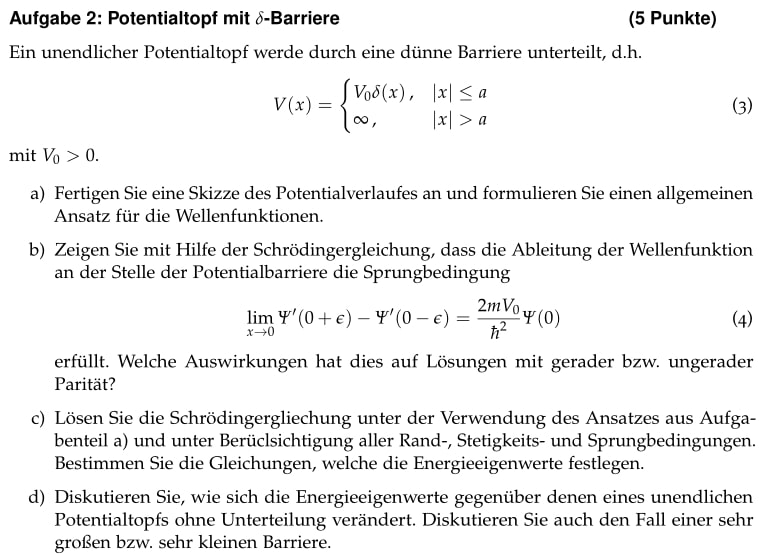
\includegraphics[width=\textwidth]{images/Aufgabe2.jpg}
        \label{fig:2}
    \end{figure}

    \subsection{a)}

    \begin{figure}[H]
        \centering
        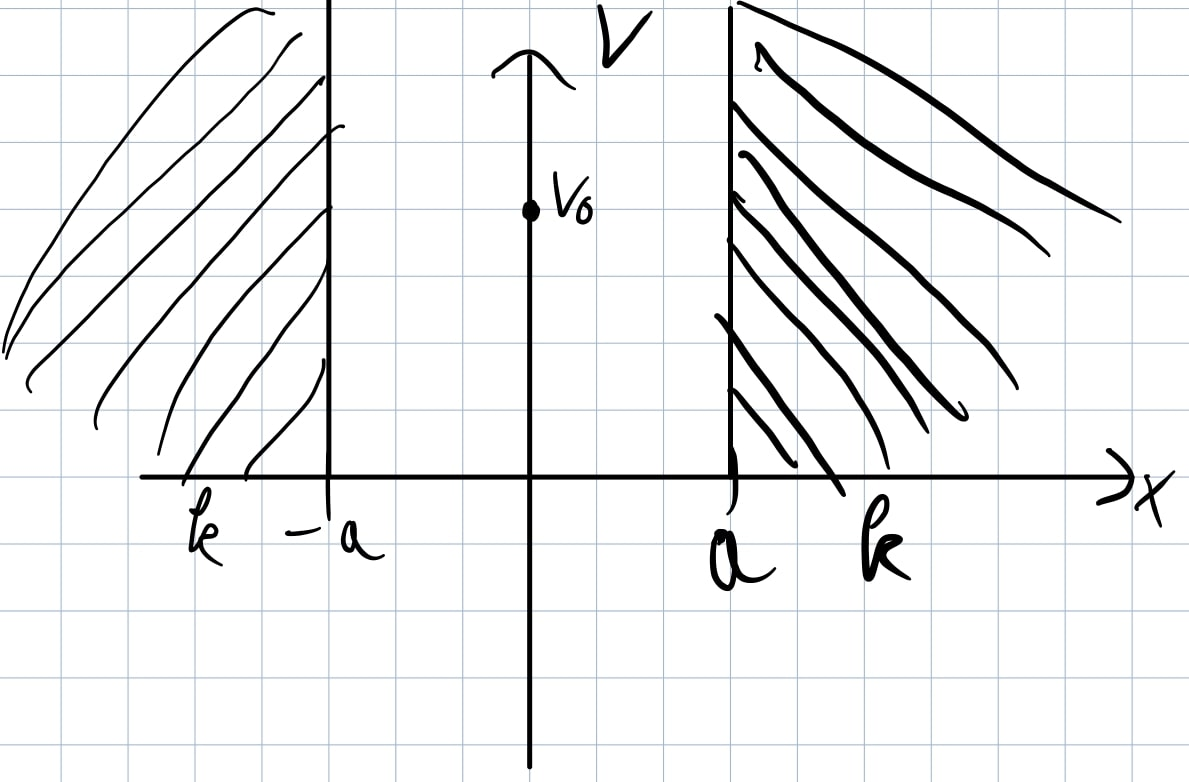
\includegraphics[width=\textwidth]{images/2a.jpg}
        \label{fig:3}
    \end{figure}

    \begin{align*}
        \intertext{Bereich $a \leq x \leq 0$:
        }
        \varphi_1(x) &= A\sin(kx) + A'\cos(kx)
        \intertext{Bereich $0 \leq x \leq a$:
        }
        \varphi_2(x) &= B\sin(kx) + B'\cos(kx)\\
        \varphi(x) &= 0 \qquad \text{sonst}
    \end{align*}

    \subsection{b)}

    \begin{align*}
        -\frac{\hbar^2}{2m} \frac{\partial^2 \varphi(x)}{\partial x^2} + V(x)\varphi(x) &= E\varphi(x) \qquad \vert \int_{-\epsilon}^{\epsilon}\,\mathrm{d}x\\
        \lim_{\epsilon \to 0} \left( \int_{-\epsilon}^{\epsilon} -\frac{\hbar^2}{2m} \frac{\partial^2 \varphi(x)}{\partial x^2} \mathrm{d}x + V_0\,\delta(x)\,\varphi(x) \mathrm{d}x \right) &= \underbrace{\lim_{\epsilon \to 0} \int_{-\epsilon}^{\epsilon} E\,\varphi(x) \mathrm{d}x}_{=0}
        \intertext{Das Integral über eine Fläche mit endlicher Höhe und infinitesimal schmaler Breite ist 0.
        }
        \lim_{\epsilon \to 0} \left[ -\frac{\hbar^2}{2m} \frac{\partial \varphi(x)}{\partial x} \right]_{-\epsilon}^{\epsilon} + V_0\,\varphi(0) &= 0\\
        \Leftrightarrow \lim_{\epsilon \to 0} \varphi'(0+\epsilon) - \varphi'(0-\epsilon) &= \frac{2m}{\hbar^2} V_0\,\varphi(0)
        \intertext{Für ungerade Parität gilt:
        }
        \varphi(x) &= -\varphi(-x)\\
        \varphi'(x) &= \varphi'(-x)\\
        \lim_{\epsilon \to 0} \varphi'(\epsilon) - \varphi'(-\epsilon) &= 0
        \intertext{Für gerade Parität gilt:
        }
        \varphi(x) &= \varphi(-x)\\
        \varphi'(x) &= -\varphi'(-x)\\
        \lim_{\epsilon \to 0} \varphi'(\epsilon) - \varphi'(-\epsilon) &= \lim_{\epsilon \to 0} 2\varphi'(\epsilon)
    \end{align*}

    \subsection{c)}

    \begin{align*}
        \varphi_1(x) &= A\sin(kx) + A'\cos(kx)\\
        \varphi_2(x) &= B\sin(kx) + B'\cos(kx)\\
        \varphi(x) &= 0 \qquad \text{sonst}
        \intertext{Fall 1:
        }\\
        \varphi_1(-a) &= -\varphi_2(a) = 0\\
        \lim_{\epsilon \to 0} \varphi'(\epsilon) - \varphi'(-\epsilon) &= 0 = \frac{2m}{\hbar^2} V_0\,\varphi(0)\\
        \varphi_1'(0) &= \varphi_2'(0)\\
        \Leftrightarrow A' &= B'\\
        \varphi(0) &= 0\\
        \Rightarrow A' &= 0 \qquad B' = 0\\
        \varphi_1(-a) &= -\varphi_2(a)\\
        A\sin(-ka) &= -B\sin(ka)\\
        \Leftrightarrow -A\sin(ka) &= -B\sin(ka)\\
        \Leftrightarrow A &= B\\
        &\varphi(x)\begin{cases}
            A\sin(kx)\; \text{für}\; -a\leq x\leq 0\\
            A\sin(kx)\; \text{für}\; 0 \leq a
        \end{cases}\\
        \Rightarrow \varphi(x) &= A\sin(kx) \qquad x\leq a\\
        \varphi(-a) &= 0\\
        \Leftrightarrow A\sin(-ka) &= 0\\
        \Rightarrow ka &=\pi n\\
        \Leftrightarrow k &= \frac{\pi n}{a} \qquad n \in \mathbb[Z]\\
        k &= \frac{\sqrt{2mE}}{\hbar}\\
        \Rightarrow \frac{\pi n}{a} &\stackrel{!}{=}  \frac{\sqrt{2mE_n}}{\hbar}\\
        \Leftrightarrow E_n &= \frac{\pi^2 \hbar^2}{2m a^2}n^2
        \intertext{Fall 2:
        }\\
        \varphi_1(-a) &= \varphi_2(a) = 0\\
        \lim_{\epsilon \to 0} \varphi_2'(\epsilon) - \varphi_1(-\epsilon) &= \frac{2mV_0}{\hbar^2} \varphi(0)\\
        &= \varphi_1(0) = \varphi_2(0)\\
        \Rightarrow A' &= B' \tag{*}\\
        \varphi_1(-a) &= \varphi_2(a)\\
        A\sin(-ka) + A'\cos(-ka) &= B\sin(ka) + B'\cos(ka) \\
        -A\sin(ka) + \underbrace{A'\cos(ka)}_{wegk"urzen} &\stackrel{(*)}{=} B\sin(ka) + \underbrace{A'\cos(ka)}_{wegk"urzen}\\
        \Rightarrow -A &= B\\
        \frac{2mV_0}{\hbar^2}A' &= \lim_{\epsilon \to 0} \left( -kA\cos(k\epsilon) - kA'\sin(k\epsilon) - kA\cos(-k\epsilon) + A'\sin(-k\epsilon) \right) \\
        \Leftrightarrow kA - kB &= A'\frac{2mV_0}{\hbar^2}\\
        \Leftrightarrow -2kA &= A'\frac{2mV_0}{\hbar^2}\\
        -\frac{A}{A'} &= \frac{2mV_0}{k\hbar^2}\\
        \varphi_1(-a) &= 0\\
        A\sin(-ka) + A'\cos(-ka) &= 0\\
        \frac{A}{A'} &= \cot(ka)\\
        -\cot(ka) &\stackrel{!}{=} \frac{mV_0}{k\hbar^2} \qquad z=ka\\
        \cot(z) &= \frac{mV_0}{\hbar^2} \frac{1}{z}a \qquad \text{numerisch lösbar}\\
        \Rightarrow z &= ka = a \cdot \frac{\sqrt{2mE}}{\hbar}\\
        \Leftrightarrow E &= \frac{\hbar^2}{2m} \left( \frac{z}{a} \right)^2
    \end{align*}

    \subsection{d)}

    \begin{align*}
        \intertext{Lösung für den unendlichen Potentialtopf:
        }
        E_n &= \frac{n^2 \hbar^2 \pi^2}{2ma^2}
        \intertext{Ungerade:
        }
        E_n &= \frac{n^2 \hbar^2 \pi^2}{2ma^2} \qquad \text{identisch}
        \intertext{Gerade:
        }
        E &= \frac{\hbar^2}{2m} \left( \frac{z}{a} \right)^2
        \intertext{Grenzfälle:
        }
        \intertext{$V_0 \to \infty$
        }
        -\cot(ka) &= \frac{mV_0}{k\hbar^2}\\
        \Leftrightarrow \tan(ka) &= -\frac{k\hbar^2}{mV_0}\\
        \Rightarrow \tan(ka) &= 0\\
        \Rightarrow ka &= n\pi\\
        \Rightarrow E_n &= \frac{\hbar^2}{2m} \frac{n^2\pi^2}{a^2}
        \intertext{Unendlicher Potentialtopf ohne Barriere
        }
        \intertext{$V_0 \to 0$
        }
        \tan(ka) &= -\frac{k\hbar^2}{mV_0} \to -\infty\\
        ka &= \pi\left( \frac{1}{2}+c \right) \qquad c \in \mathbb{Z}\\
        \Leftrightarrow k &= \frac{\pi}{a}\left( \frac{1}{2}+c \right)\\
        \frac{\pi}{a}\left( \frac{1}{2}+c \right) &\stackrel{!}{=} \frac{\sqrt{2mE}}{\hbar}\\
        \Leftrightarrow E &= \frac{\pi^2}{a^2}\frac{\hbar}{2m} \left( \frac{1}{2}+c \right)
    \end{align*}

\section{Aufgabe 3}

    \begin{figure}[H]
        \centering
        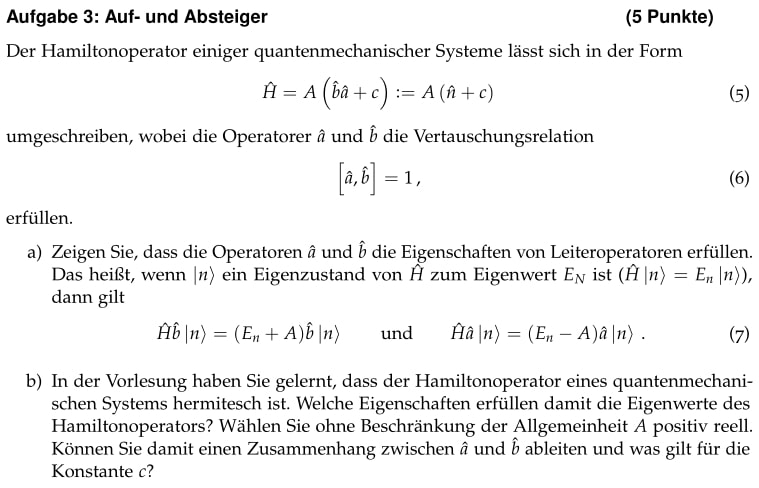
\includegraphics[width=\textwidth]{images/Aufgabe3ab.jpg}
        \label{fig:4}
    \end{figure}
    \begin{figure}[H]
        \centering
        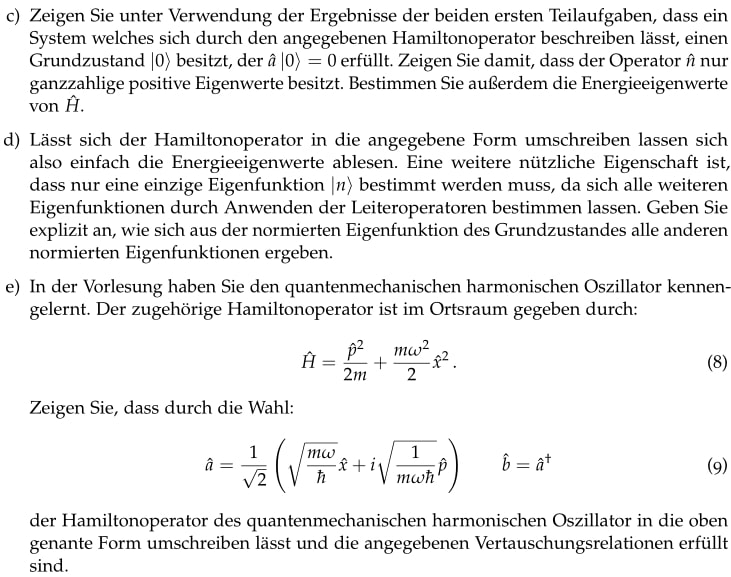
\includegraphics[width=\textwidth]{images/Aufgabe3cde.jpg}
        \label{fig:5}
    \end{figure}

    \subsection{a)}

    \begin{align*}
        \hat{H} &= A\left( \hat{b}\hat{a} + c \right)\\
        \left[ \hat{a}, \hat{b} \right] &= 1\\
        \Rightarrow \hat{a}\hat{b} - \hat{b}\hat{a} &= 1\\
        \Leftrightarrow \hat{a}\hat{b} &= \hat{b}\hat{a} + 1\\
        \Leftrightarrow \hat{b}\hat{a} &= \hat{a}\hat{b} - 1\\
        \\
        \hat{H}\hat{b} \vert n \rangle &\stackrel{!}{=} A\left( \hat{b}\hat{a} +c \right)\hat{b} \vert n \rangle\\
        &= A\left(\hat{b}\hat{a}\hat{b}+c\hat{b} \right) \vert n \rangle\\
        &= A\hat{b} \left( \underline{\hat{a}\hat{b}} +c \right) \vert v \rangle\\
        &\stackrel{!}{=} A\hat{b} \left( \underline{\hat{b}\hat{a} + 1} + c \right) \vert n \rangle\\
        \Leftrightarrow &= \hat{b} \left(\underbrace{A\left(\hat{b}\hat{a}+c \right)}_{=\hat{H}} + A \right) \vert n \rangle\\
        &= \hat{b} \left( \hat{H} + A \right) \vert n \rangle\\
        &= \left( E_N + A \right) \hat{b} \vert n \rangle\\
        \\
        \hat{H}\hat{a} \vert n \rangle &\stackrel{!}{=} A\left( \hat{b}\hat{a} +c \right)\hat{a} \vert n \rangle\\ 
        &= A\left(\hat{b}\hat{a}\hat{a}+c\hat{a} \right) \vert n \rangle\\
        &= A\hat{a} \left( \underline{\hat{b}\hat{a}} +c \right) \vert n \rangle\\
        &\stackrel{!}{=} A\hat{a} \left( \underline{\hat{a}\hat{b} - 1} + c \right) \vert n \rangle\\
        \Leftrightarrow &= \hat{a} \left(\underbrace{A\left(\hat{a}\hat{b}+c \right)}_{\neq\hat{H}} - A \right) \vert n \rangle\\
        &= \hat{a} \left( \hat{H} - A \right) \vert n \rangle\\
        &= \left( E_N - A \right) \hat{a} \vert n \rangle
    \end{align*}

    \subsection{b)}

    \subsection{c)}

    \subsection{d)}

    \subsection{e)}

\end{document}